%<dscrpt>Fichier de déclarations Latex à inclure au début d'un élément de cours.</dscrpt>

\documentclass[a4paper]{article}
\usepackage[hmargin={1.8cm,1.8cm},vmargin={2.4cm,2.4cm},headheight=13.1pt]{geometry}

%includeheadfoot,scale=1.1,centering,hoffset=-0.5cm,
\usepackage[pdftex]{graphicx,color}
\usepackage[french]{babel}
%\selectlanguage{french}
\addto\captionsfrench{
  \def\contentsname{Plan}
}
\usepackage{fancyhdr}
\usepackage{floatflt}
\usepackage{amsmath}
\usepackage{amssymb}
\usepackage{amsthm}
\usepackage{stmaryrd}
%\usepackage{ucs}
\usepackage[utf8]{inputenc}
%\usepackage[latin1]{inputenc}
\usepackage[T1]{fontenc}


\usepackage{titletoc}
%\contentsmargin{2.55em}
\dottedcontents{section}[2.5em]{}{1.8em}{1pc}
\dottedcontents{subsection}[3.5em]{}{1.2em}{1pc}
\dottedcontents{subsubsection}[5em]{}{1em}{1pc}

\usepackage[pdftex,colorlinks={true},urlcolor={blue},pdfauthor={remy Nicolai},bookmarks={true}]{hyperref}
\usepackage{makeidx}

\usepackage{multicol}
\usepackage{multirow}
\usepackage{wrapfig}
\usepackage{array}
\usepackage{subfig}


%\usepackage{tikz}
%\usetikzlibrary{calc, shapes, backgrounds}
%pour la présentation du pseudo-code
% !!!!!!!!!!!!!!      le package n'est pas présent sur le serveur sous fedora 16 !!!!!!!!!!!!!!!!!!!!!!!!
%\usepackage[french,ruled,vlined]{algorithm2e}

%pr{\'e}sentation du compteur de niveau 2 dans les listes
\makeatletter
\renewcommand{\labelenumii}{\theenumii.}
\renewcommand{\thesection}{\Roman{section}.}
\renewcommand{\thesubsection}{\arabic{subsection}.}
\renewcommand{\thesubsubsection}{\arabic{subsubsection}.}
\makeatother


%dimension des pages, en-t{\^e}te et bas de page
%\pdfpagewidth=20cm
%\pdfpageheight=14cm
%   \setlength{\oddsidemargin}{-2cm}
%   \setlength{\voffset}{-1.5cm}
%   \setlength{\textheight}{12cm}
%   \setlength{\textwidth}{25.2cm}
   \columnsep=1cm
   \columnseprule=0.5pt

%En tete et pied de page
\pagestyle{fancy}
\lhead{MPSI-\'Eléments de cours}
\rhead{\today}
%\rhead{25/11/05}
\lfoot{\tiny{Cette création est mise à disposition selon le Contrat\\ Paternité-Pas d'utilisations commerciale-Partage des Conditions Initiales à l'Identique 2.0 France\\ disponible en ligne http://creativecommons.org/licenses/by-nc-sa/2.0/fr/
} }
\rfoot{\tiny{Rémy Nicolai \jobname}}


\newcommand{\baseurl}{http://back.maquisdoc.net/data/cours\_nicolair/}
\newcommand{\urlexo}{http://back.maquisdoc.net/data/exos_nicolair/}
\newcommand{\urlcours}{https://maquisdoc-math.fra1.digitaloceanspaces.com/}

\newcommand{\N}{\mathbb{N}}
\newcommand{\Z}{\mathbb{Z}}
\newcommand{\C}{\mathbb{C}}
\newcommand{\R}{\mathbb{R}}
\newcommand{\D}{\mathbb{D}}
\newcommand{\K}{\mathbf{K}}
\newcommand{\Q}{\mathbb{Q}}
\newcommand{\F}{\mathbf{F}}
\newcommand{\U}{\mathbb{U}}
\newcommand{\p}{\mathbb{P}}


\newcommand{\card}{\mathop{\mathrm{Card}}}
\newcommand{\Id}{\mathop{\mathrm{Id}}}
\newcommand{\Ker}{\mathop{\mathrm{Ker}}}
\newcommand{\Vect}{\mathop{\mathrm{Vect}}}
\newcommand{\cotg}{\mathop{\mathrm{cotan}}}
\newcommand{\sh}{\mathop{\mathrm{sh}}}
\newcommand{\ch}{\mathop{\mathrm{ch}}}
\newcommand{\argsh}{\mathop{\mathrm{argsh}}}
\newcommand{\argch}{\mathop{\mathrm{argch}}}
\newcommand{\tr}{\mathop{\mathrm{tr}}}
\newcommand{\rg}{\mathop{\mathrm{rg}}}
\newcommand{\rang}{\mathop{\mathrm{rg}}}
\newcommand{\Mat}{\mathop{\mathrm{Mat}}}
\newcommand{\MatB}[2]{\mathop{\mathrm{Mat}}_{\mathcal{#1}}\left( #2\right) }
\newcommand{\MatBB}[3]{\mathop{\mathrm{Mat}}_{\mathcal{#1} \mathcal{#2}}\left( #3\right) }
\renewcommand{\Re}{\mathop{\mathrm{Re}}}
\renewcommand{\Im}{\mathop{\mathrm{Im}}}
\renewcommand{\th}{\mathop{\mathrm{th}}}
\newcommand{\repere}{$(O,\overrightarrow{i},\overrightarrow{j},\overrightarrow{k})$}
\newcommand{\cov}{\mathop{\mathrm{Cov}}}

\newcommand{\absolue}[1]{\left| #1 \right|}
\newcommand{\fonc}[5]{#1 : \begin{cases}#2 \rightarrow #3 \\ #4 \mapsto #5 \end{cases}}
\newcommand{\depar}[2]{\dfrac{\partial #1}{\partial #2}}
\newcommand{\norme}[1]{\left\| #1 \right\|}
\newcommand{\se}{\geq}
\newcommand{\ie}{\leq}
\newcommand{\trans}{\mathstrut^t\!}
\newcommand{\val}{\mathop{\mathrm{val}}}
\newcommand{\grad}{\mathop{\overrightarrow{\mathrm{grad}}}}

\newtheorem*{thm}{Théorème}
\newtheorem{thmn}{Théorème}
\newtheorem*{prop}{Proposition}
\newtheorem{propn}{Proposition}
\newtheorem*{pa}{Présentation axiomatique}
\newtheorem*{propdef}{Proposition - Définition}
\newtheorem*{lem}{Lemme}
\newtheorem{lemn}{Lemme}

\theoremstyle{definition}
\newtheorem*{defi}{Définition}
\newtheorem*{nota}{Notation}
\newtheorem*{exple}{Exemple}
\newtheorem*{exples}{Exemples}


\newenvironment{demo}{\renewcommand{\proofname}{Preuve}\begin{proof}}{\end{proof}}
%\renewcommand{\proofname}{Preuve} doit etre après le begin{document} pour fonctionner

\theoremstyle{remark}
\newtheorem*{rem}{Remarque}
\newtheorem*{rems}{Remarques}

\renewcommand{\indexspace}{}
\renewenvironment{theindex}
  {\section*{Index} %\addcontentsline{toc}{section}{\protect\numberline{0.}{Index}}
   \begin{multicols}{2}
    \begin{itemize}}
  {\end{itemize} \end{multicols}}


%pour annuler les commandes beamer
\renewenvironment{frame}{}{}
\newcommand{\frametitle}[1]{}
\newcommand{\framesubtitle}[1]{}

\newcommand{\debutcours}[2]{
  \chead{#1}
  \begin{center}
     \begin{huge}\textbf{#1}\end{huge}
     \begin{Large}\begin{center}Rédaction incomplète. Version #2\end{center}\end{Large}
  \end{center}
  %\section*{Plan et Index}
  %\begin{frame}  commande beamer
  \tableofcontents
  %\end{frame}   commande beamer
  \printindex
}


\makeindex
\begin{document}
\noindent

\debutcours{Matrices : transformations élémentaires}{0.4 \tiny{le \today}}

\section{Algorithmes}
\subsection{Algorithme de Gauss} \index{algorithme de Gauss}
\subsubsection{Opérations élémentaires}
\index{opérations élémentaires} On appelle \emph{opérations élémentaires} les transformations suivantes d'une matrice à $p$ lignes et $q$ colonnes en une matrice à $p$ lignes et $q$ colonnes.
\begin{itemize}
 \item Permuter deux lignes.
 \item Permuter deux colonnes.
 \item Pour $i$ et $i'$ entre $1$ et $p$ et $\lambda$ scalaire quelconque: ajouter à la ligne $i$ la ligne $i'$ multipliée par $\lambda$. Bien noter que seule la ligne $i$ est modifiée.
 \item Pour $j$ et $j'$ entre $1$ et $q$ et $\lambda$ scalaire quelconque: ajouter à la colonne $j$ la colonne $j'$ multipliée par $\lambda$. Bien noter que seule la colonne $j$ est modifiée.
 \item Multiplier une ligne par un scalaire $\lambda$ \emph{non nul}.
 \item Multiplier une colonne par un scalaire $\lambda$ \emph{non nul}.
\end{itemize}
Les opérations élémentaires sont \emph{réversibles}; c'est à dire que si $A$ est la matrice de départ et $A'$ une matrice obtenue à partir de $A$ par une opération élémentaire, on peut, par opération élémentaire, transformer $A'$ en $A$. Par exemple, pour le troisième type, il suffit d'ajouter $-\lambda$ fois la ligne $i'$ à la ligne $i$.
\subsubsection{Principe général}
L'algorithme de Gauss transforme une matrice en utilisant \emph{exclusivement} des opérations élémentaires.\newline
Le diagramme de la figure \ref{fig:C2234_1} présente un algorithme de Gauss très général utilisant des procédures \verb|Pivot|, \verb|Nettoie| et \verb|Permute|. Les diverses variantes s'obtiennent en modifiant ces procédures.
\begin{figure}[h!t]
 \centering
 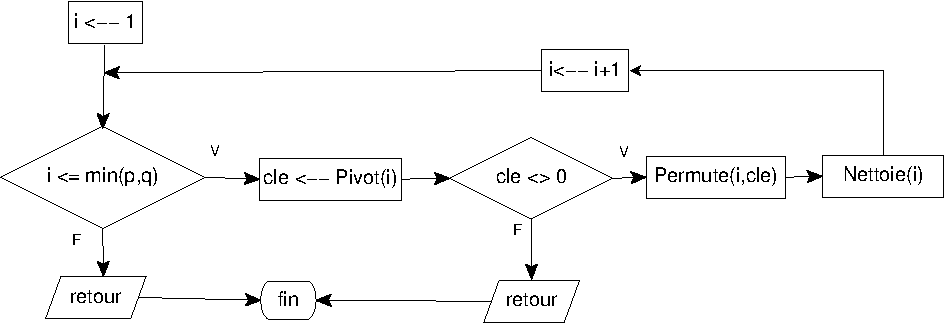
\includegraphics{C2234_1.pdf}
 \caption{Algorithme de Gauss}
 \label{fig:C2234_1}
\end{figure}
Un tableau à deux dimensions représente une matrice à $p$ lignes et $q$ colonnes. Il est commode d'utiliser des variables globales (par exemple \verb|A|, \verb|p|, \verb|q|) pour désigner le tableau et ses dimensions. Les variables \verb|i| et \verb|cle| sont locales. \medskip
\begin{itemize}
  \item La procédure \verb|Pivot(i)| renvoie une clé (pas une valeur mais un indice ou un couple d'indices) du tableau dont la valeur (appelée \emph{pivot})\index{pivot} est non nulle. Cette clé est cherchée dans une partie de la matrice. Plusieurs stratégies sont possibles pour le choix de cette clé.\medskip
  \item La procédure \verb|Permute(i,cle)| échange des lignes (et éventuellement des colonnes) pour placer la valeur pivot en position $(i,i)$.\medskip
  \item La procédure \verb|Nettoie| fait apparaitre des $0$ dans une partie de la colonne $i$. Pour cela elle utilise exclusivement des transformations élémentaires du type
$L_j \longleftarrow L_j + \lambda L_i$. \medskip
\end{itemize}
\begin{figure}[ht]
 \centering
 \input{C2234_2.pdf_t}
 \caption{Procédure \og Nettoie\fg pour l'algorithme I}
 \label{fig:C2234_2}
\end{figure}
Les procédures, la forme de la matrice finale et ce que renvoie l'algorithme sont précisés dans les variantes.\newline
Il est important de noter que l'algorithme s'arrête soit parce que $i$ dépasse $\min(p,q)$ soit parce que la recherche d'un pivot non nul échoue.

\subsection{Algorithme I : pivot partiel}
\index{algorithme du pivot partiel}
La procédure \verb|Pivot(i)| cherche une valeur pivot non nulle dans la bas de la colonne courante c'est dire parmi les termes $a_{i,i},a_{i+1,i},\cdots a_{p,i}$. Si elle n'en trouve pas elle renvoie une valeur conventionnelle.\newline
Différentes stratégies doivent être adoptées suivant le contexte.
\begin{itemize}
  \item Pour un calcul dans $\Q$ \og à la main\fg, on préfèrera une valeur pivot comme $1$ ou $-1$.
  \item Pour un calcul numérique, il vaut mieux choisir le pivot le plus grand possible afin de minimiser les erreurs d'arrondi.
  \item Pour un calcul formel avec un paramètre $\lambda$, il faut choisir une valeur où $\lambda$ ne figure pas afin de ne pas avoir à imposer de condition sur le paramètre. 
\end{itemize}

La procédure \verb|Nettoie| (figure \ref{fig:C2234_2}) fait apparaitre des $0$ dans le bas de la colonne courante. Pour cela elle effectue
\[
 L_{i'}\leftarrow L_{i'}-\frac{a_{i',i}}{a_{i,i}}L_i \hspace{0.5cm} \text{ pour } i' \text{ de } i+1 \text{ à } p.
\]
Trois formes sont possibles pour la matrice finale suivant que l'algorithme termine avec $i>p$, $i>q$ ou par l`échec de la recherche d'un pivot non nul. 
\[
 \begin{bmatrix}
\neq 0 &   .     &        &        & . & . \\
0      & \neq 0  &        &        & . & . \\
\vdots &         & \ddots &        & . & . \\
0      &\cdots  &     0   &\neq 0  & . & .
 \end{bmatrix}
\hspace{1cm} 
 \begin{bmatrix}
\neq 0&       &       &  \\
 0    &\neq 0 &       &  \\
      & 0     &\ddots &  \\
\vdots&       &\ddots & \neq 0 \\
      &       &       &  \\
 0    &       &       & 0
 \end{bmatrix}
\hspace{1cm}
\begin{bmatrix}
 \neq 0 &  &  &  &  &  \\
 0 & \ddots &  &  &  &  \\
 \vdots &\ddots  &\neq 0  &  &  &  \\
        &        &0  &0  &  &  \\
        &        &\vdots & \vdots & . & . \\
 0      &        &   0   &   0    & . &. 
\end{bmatrix}.
\]

\subsection{Algorithme I' : pivot partiel étendu}
\index{algorithme du pivot partiel étendu} La différence avec la version I porte uniquement sur \verb|Nettoie|. L'appel \verb|Nettoie(i)| effectue
\[
\begin{aligned}
  &\text{Pour \emph{tous} les $i'$ de $1$ à $p$ sauf $i$}, \hspace{0.5cm} L_{i'}\leftarrow L_{i'}-\frac{a_{i',i}}{a_{i,i}}L_i \\
  &\text{Pour la ligne $i$}, \hspace{0.5cm} L_{i}\leftarrow \frac{1}{a_{i,i}}L_i
\end{aligned}
\]
Ainsi la colonne $i$ ne contient que des $0$ sauf un $1$ en position $i,i$.\newline
La forme de la matrice finale est, pour les trois cas possibles,
\[
 \begin{bmatrix}
1      &   0   &        & 0      & . & . \\
0      & 1     &        & \vdots & . & . \\
\vdots &       & \ddots & 0 & .  & . & \\
0      &\cdots &    0   & 1 & .  & . &
 \end{bmatrix}
\hspace{1cm} 
 \begin{bmatrix}
1 &       &       &  \\
 0    &1 &       &  \\
      & 0     &\ddots &  \\
\vdots&       &\ddots & 1 \\
      &       &       &  \\
 0    &       &       & 0
 \end{bmatrix}
\hspace{1cm}
\begin{bmatrix}
 1     &        &0      &       &  &  \\
 0     & \ddots &       &       &  &  \\
\vdots & \ddots &1      &       &  &  \\
       &        &0      & 0     &  &  \\
       &        &\vdots &\vdots & . & . \\
 0     &        &   0   &   0   & . &. 
\end{bmatrix}.
\]

\index{algorithme du pivot total}
\subsection{Algorithme II : pivot total}
L'algorithme du pivot total se différencie des algorithmes précédents par la zone de recherche du pivot non nul et par la procédure de permutation qui peut agir sur les colonnes.\newline
L'appel \verb|Pivot(i)| cherche une valeur pivot non nulle dans tout le bas de la matrice et pas seulement dans la colonne $i$. La procédure renvoie donc un couple $(i_0,j_0)$ tel que $i\leq i_0\leq p$, $i\leq j_0 \leq q$ et $a_{i_0,j_0}\neq 0$ ou bien une valeur conventionnelle si elle n'en trouve pas.\newline
La procédure de permutation échange les lignes $i$ et $i_0$ et les \emph{colonnes} $i$ et $j_0$ de manière à placer la valeur pivot non nulle en position $i,i$.\newline
La procédure de nettoyage est la même que pour le pivot partiel.\newline
La matrice à la fin de l'algorithme est de l'une des formes suivantes  
\[
 \begin{bmatrix}
\neq 0 &   .     &        &        & . & . \\
0      & \neq 0  &        &        & . & . \\
\vdots &         & \ddots &        & . & . \\
0      &\cdots  &     0   &\neq 0  & . & .
 \end{bmatrix}
\hspace{1cm} 
 \begin{bmatrix}
\neq 0&       &       &  \\
 0    &\neq 0 &       &  \\
      & 0     &\ddots &  \\
\vdots&       &\ddots & \neq 0 \\
      &       &       &  \\
 0    &       &       & 0
 \end{bmatrix}
\hspace{1cm}
\begin{bmatrix}
 \neq 0 &  &  &  &  &  \\
 0 & \ddots &  &  &  &  \\
 \vdots &\ddots  &\neq 0 & .& .& . \\
        &        &0      &0 & \cdots &  0\\
        &        &\vdots & \vdots &  &\vdots  \\
 0      &        &   0   &   0    & \cdots & 0
\end{bmatrix}.
\]

\section{Matrices et opérations élémentaires}
\index{matrices d'opérations élémentaires}
\begin{defi}[matrices d'opérations élémentaires]
 Soit $n \in \N^*$ et $(i,j)\in \llbracket 1,n \rrbracket^2$. Toutes les matrices définies ici appartiennent à $\mathcal{M}_n(\K)$. Elles sont obtenues par des transformations élémentaires de la matrice identité $I_n$.\medskip
\begin{itemize}
 \item $P_{i,j}(n)$ est obtenue à partir de $I_n$ en échangeant les lignes $i$ et $j$.\medskip
 \item $A_{i,j,\lambda}(n)$ est obtenue à partir de $I_n$ en ajoutant à la ligne $i$ la ligne $j$ multipliée par $\lambda$ (scalaire quelconque).\medskip 
 \item $D_{i,\lambda}(n)$ est obtenue à partir de $I_n$ en multipliant par $\lambda$ (scalaire non nul) la ligne $i$ de $I_n$. 
\end{itemize}
\end{defi}
\begin{rem}
 La matrice $A_{i,j,\lambda}(n)$ ne différe de $I_n$ que par le terme $i,j$ qui est égal à $\lambda$ au lieu de $0$. Elle est triangulaire supérieure si $i < j$ et triangulaire inférieure si $j < i$.
\end{rem}
\noindent La proposition suivante traduit les opérations élémentaires en termes de multiplications matricielles. Une opération élémentaire portant sur les lignes est obtenue par multiplication \emph{à gauche} par une matrice d'opérations élémentaires. Les opérations portant sur les colonnes sont obtenues par multiplication \emph{à droite}.
\begin{prop}
 Soit $M\in \mathcal M_{p,q}(\K)$. Les entiers $i$ et $j$ sont entre $1$ et $p$ quand ils figurent dans une matrice placée à gauche et entre $1$ et $q$ quand ils figurent dans une matrice placée à droite.  \medskip
\begin{itemize}
 \item $P_{i,j}(p)M$ est obtenue à partir de $M$ en permutant les lignes $i$ et $j$.\medskip
 \item $MP_{i,j}(q)$ est obtenue à partir de $M$ en permutant les colonnes $i$ et $j$.\medskip
 \item $A_{i,j,\lambda}(p)M$ est obtenue à partir de $M$ en remplaçant $L_i(M)$ par $L_i(M)+\lambda L_j(M)$ où $\lambda \in \K$ .\medskip
 \item $MA_{i,j,\lambda}(p)$ est obtenue à partir de $M$ en remplaçant $C_j(M)$ par $C_j(M)+\lambda C_i(M)$ où $\lambda \in \K$.\medskip
 \item $D_{i,\lambda}(p)M$ est obtenue à partir de $M$ en multipliant la ligne $i$ par $\lambda$ (scalaire non nul).\medskip
 \item $MD_{i,\lambda}(q)$ est obtenue à partir de $M$ en multipliant la colonne $i$ par $\lambda$ (scalaire non nul).
\end{itemize}
\end{prop}
\begin{demo}
 On vérifie à partir de la définition du produit matriciel. Il est utile de remarquer que les lignes de $A_{i,j,\lambda}(p)$ sont celles de $I_p$ sauf la $i$-eme et que les colonnes de $A_{i,j,\lambda}(q)$ sont celles de $I_q$ sauf la $j$-eme.
\end{demo}
\begin{prop}
 Toutes les matrices de transformations élémentaires sont inversibles avec 
\[
 P_{i,j}(p)^{-1}=P_{i,j}(p),\hspace{0.5cm} A_{i,j,\lambda}(n)^{-1}=A_{i,j,-\lambda}(n),\hspace{0.5cm}
D_{i,\lambda}(n)^{-1}=D_{i,\frac{1}{\lambda}}(n).
\]
\end{prop}
\begin{demo}
 C'est facile en utilisant l'effet d'une multiplication par une matrice élémentaire.
\end{demo}
\begin{rems}
\begin{enumerate}
  \item La définition des matrices élémentaires à l'aide d'opérations élémentaires correspond aux relations triviales
\[ 
P_{i,j}(p) = P_{i,j}(p)\, I_p = I_p P_{i,j}(p),\hspace{0.5cm} A_{i,j,\lambda}(p) = A_{i,j,\lambda}(p)\,I_p,\hspace{0.5cm} D_{i,\lambda}(p) = D_{i,\lambda}(p)\, I_p. 
\]
  \item Si une matrice $B$ est obtenue à partir de $A$ par une opération élémentaire, alors $A$ et $B$ sont équivalentes. Par transitivité, si $B$ est obtenue par une succession de transformations élémentaires alors $B$ est équivalente à $A$.
\end{enumerate}
\end{rems}

\index{invariant par transformation élémentaire} Un invariant par transformation élémentaire est un nombre (ou plus généralement un objet mathématique) attaché à une matrice et qui est conservé par une transformation élémentaire.
\begin{prop}
  Le noyau d'une matrice est un invariant par opérations élémentaires sur les lignes.\newline
  L'image d'une matrice est un invariant par opérations élémentaires sur les colonnes.\newline
  Le rang est un invariant par opérations élémentaires.
\end{prop}
\begin{demo}
Soit $A$ et $B$ dans $\mathcal{M}_{p, q}(\K)$.\newline
Si $B$ est obtenue par transformations élémentaires sur les lignes à partir de $A$, il existe $P$ qui est un produit de matrices élémentaires telle que $B = PA$. Un produit de matrices inversibles est inversible donc $P$ est inversible. Alors:
\[
 \forall X \in \mathcal{M}_{p,1}(\K),\hspace{0.5cm}
 X \in \ker B \Leftrightarrow BX = 0_{\mathcal{M}_{p,1}(\K)} 
 \Leftrightarrow P A X = 0_{\mathcal{M}_{p,1}(\K)}
 \Leftrightarrow A X = 0_{\mathcal{M}_{p,1}(\K)}
\]
car $P$ est inversible.\newline
Si $B$ est obtenue par transformations élémentaires sur les colonnes à partir de $A$, il existe $Q$ qui est un produit de matrices élémentaires telle que $B = AQ$. Un produit de matrices inversibles est inversible donc $Q$ est inversible. Alors:
\[
 \Im B = \left\lbrace B X\text{ avec } X \in \mathcal{M}_{p,1}(\K)\right\rbrace 
 = \left\lbrace A (Q X)\text{ avec } X \in \mathcal{M}_{p,1}(\K)\right\rbrace
 = \left\lbrace A Y\text{ avec } Y \in \mathcal{M}_{p,1}(\K)\right\rbrace
\]
car $Q$ étant inversible, $\left\lbrace Q X\text{ avec } X \in \mathcal{M}_{p,1}(\K)\right\rbrace = \mathcal{M}_{p,1}(\K)$.\newline
Le rang d'une matrice est la dimension de son image. Il est invariant par équivalence. Le rang est donc invariant par les opérations sur les colonnes car $B$ est équivalent à $A$ si elle est obtenue par des transformations élémentaires de $A$.\newline
Comme le sous-espace vectoriel noyau est invariant par opérations sur les lignes, sa dimension est aussi invariante. Avec le théorème du rang, on en déduit que le rang est aussi invariant par opérations sur les lignes. C'est donc un invariant pour toutes les opérations élémentaires. C'est aussi une conséquence de la remarque 2 au dessus.
\end{demo}
\begin{prop}
Pour des matrices carrées, l'inversibilité (c'est à dire le caractère inversible ou non) est un invariant par opérations élémentaires.
\end{prop}
\begin{demo}
Soit $A \in \mathcal{M}_{p}(\K)$. La matrice $A$ est inversible si et seulement si $\rg(A) = p$. L'invariance du rang entraine donc l'invariance de l'inversibilité.
\end{demo}

\section{Applications}
\subsection{Pivot partiel}
\begin{prop}[Inversibilité d'une matrice carrée]
 Une matrice carrée $A\in \mathcal{M}_p(\K)$ est inversible si et seulement si la matrice obtenue à partir de $A$ par l'algorithme I est de la forme
\begin{displaymath} T =
  \begin{bmatrix}
\neq 0 &        &        &        \\
0      & \neq 0  &        &        \\
\vdots &         & \ddots &        \\
0      &\cdots  &     0   &\neq 0 
 \end{bmatrix}
\end{displaymath}
\end{prop}
\begin{demo}
 L'algorithme I conduit à une matrice $PA$ avec $P$ inversible car égal à un produit de matrices élémentaires. Si $PA$ est de la forme $T$, comme $T$ est inversible (triangulaire supérieure avec des termes non nuls sur la diagonale), $A$ est également inversible.\newline
Si $PA$ n'est pas de la forme $T$, elle est de la forme
\[
T'=
 \begin{bmatrix}
 \neq 0 &  &  &  &  &  \\
 0 & \ddots &  &  &  &  \\
 \vdots &\ddots  &\neq 0  &  &  &  \\
        &        &0  &0  &  &  \\
        &        &\vdots & \vdots & . & . \\
 0      &        &   0   &   0    & . &. 
\end{bmatrix} 
\]
qui n'est pas inversible car triangulaire supérieure avec des termes nuls sur la diagonale. On en déduit que $A$ n'est pas inversible.
\end{demo}

\subsection{Pivot partiel étendu}
\begin{prop}[Résolution d'une équation linéaire]
 Soit $A\in \text{GL}_p(\K)$ et $Y\in \mathcal{M}_{p,1}(\K)$. Il existe un unique vecteur colonne $X$ tel que $AX=Y$ (système de Cramer)\index{système de Cramer}. Pour l'obtenir, on forme une matrice par blocs à $p+1$ colonnes et on utilise l'algorithme du pivot partiel étendu.
\begin{displaymath}
\left[ A \; Y\right] \xrightarrow{\text{Algorithme I'}} \left[ I_p\; X\right] 
\end{displaymath}
\end{prop}
\begin{demo}
 Comme $A$ est inversible, l'unique solution $X$ de $A X = Y$ est $A^{-1} Y$.\newline
 Les opérations élémentaires intervenant dans l'algorithme du pivot partiel étendu (I') sont les mêmes que l'on parte de $A$ ou de $[A\;X]$. Notons $P_1, P_2,\cdots P_s$ les matrices élémentaires correspondant à ces opérations. L'algorithme n'opère que sur les lignes et ces opérations sont associées à des multiplications par des matrices élémentaires placées à gauche :
\[
 I_p  = P_s\,P_{s-1}\cdots P_2\,P_1\,A \Rightarrow A^{-1} = P_s\,P_{s-1}\cdots P_2 \, P_1 
 \Rightarrow X = A^{-1}\,Y = P_s\,P_{s-1}\cdots P_2 \, P_1\, Y .
\]
Autrement dit, la solution $X$ s'obtient à partir de $Y$ en lui faisant subir les \emph{mêmes} opérations élémentaires que celles permettant de passer de $A$ à $I_p$. En écrivant $Y$ à droite de $A$, cela se réalise automatiquement sans qu'il soit nécessaire de mémoriser ces transformations élémentaires.
\end{demo}

\begin{rem}
 On a vu dans le cours sur les matrices pour elles mêmes que calculer $A^{-1}$ c'est exprimer les colonnes canoniques $X_1, \cdots, X_p$ en fonction des colonnes de $A$. Cela revient à résoudre les $p$ systèmes de Cramer analogues au précédent en remplaçant le second membre $Y$ par $X_1, \cdots, X_q$. On peut donc modifier la proposition précédente pour calculer la matrice inverse.
\end{rem}

\begin{prop}[Inversion d'une matrice carrée inversible]
 Soit $A\in \mathcal{M}_p(\K)$ inversible. On forme une matrice par blocs dans $\mathcal{M}_{p,2p}(\K)$ en plaçant à droite de $A$ un bloc constitué de la matrice identité. L'algorithme du pivot partiel étendu (I') conduit à une matrice dont le bloc de droite est $A^{-1}$.
\begin{displaymath}
\left[ A \; I_p\right] \xrightarrow{\text{Algorithme I'}} \left[ I_p\; A^{-1}\right] 
\end{displaymath}
\end{prop}
\begin{demo}
 Avec les mêmes notations que dans la démonstration de la proposition précédente,
\[
A^{-1} = P_s\,P_{s-1}\cdots P_2 \, P_1 = P_s\,P_{s-1}\cdots P_2 \, P_1\, I_p. 
\]
Autrement dit, $A^{-1}$ s'obtient à partir de $I_p$ en lui faisant subir les \emph{mêmes} transformations élémentaires que celles permettant de passer de $A$ à $I_p$. En écrivant $I_p$ à droite de $A$ dans une matrice par blocs, cela se réalise automatiquement sans qu'il soit nécessaire de mémoriser les transformations élémentaires.
\end{demo}

\begin{rem}
 Attention, cette méthode pour inverser une matrice est très séduisante mais il ne faut pas chercher à l'appliquer systématiquement. Lorsqu'on fait des calculs à la main, les éventuelles erreurs de calcul sont difficiles à trouver.\newline
 Les autres méthodes à considérer reviennent à résoudre des systèmes d'équations.
\begin{itemize}
 \item Résoudre un système de $p$ équations à $p$ inconnues $AX=Y$ avec une colonne $X$ inconnue et une colonne $Y$ formelle. La matrice inverse se lira sur l'expression des solutions en fonction des paramètres formels.
 \item Exprimer les colonnes canoniques $X_1, \cdots, X_p$ en fonction des colonnes $C_1(A), \cdots, C_p(A)$. Cela revient à résoudre un système de $p$ équations matricielles.
\end{itemize}
Selon les cas, l'une ou l'autre de ces méthodes est plus facile à mettre en \oe{}uvre.
\end{rem}
\begin{rems}[mauvaises idées]
Pour résoudre un système de Cramer $AX = Y$, on peut être tenté de calculer d'abord la matrice inverse $A^{-1}$ puis d'effectuer la multiplication $Y = A^{-1}\, X$. C'est absurde du point de vue de la complexité car inverser une matrice $p\times p$ c'est résoudre $p$ systèmes de Cramer au lieu d'un (sans compter la multiplication matricielle ensuite).\newline
Une autre mauvaise idée est d'utiliser des coefficients indéterminés ($p^2$) pour inverser une matrice en cherchant à résoudre le système de $p^2$ équations linéaires à $p^2$ inconnues obtenues en identifiant les coefficients du produit avec ceux de $I_p$. 
\end{rems}

\subsection{Pivot total}
\begin{prop}[Calcul d'un rang]
 Le rang d'une matrice $A$ est le nombre de termes non nuls sur la diagonale de la matrice obtenue à partir de $A$ par l'algorithme du pivot total.
\end{prop}
\begin{demo}
 Le rang est invariant par opération élémentaire. Le rang de la matrice obtenue par les opérations élementaires de l'algorithme du pivot total est le nombre de termes non nuls sur la diagonale.
\end{demo}
\begin{rem}
 Soit $r$ le rang d'une matrice $A\in \mathcal{M}_{p,q}(\K)$. On peut obtenir $J_r(p,q)$ par des opérations élémentaires à partir de $A$ en complétant l'algorithme du pivot total. D'abord on fait comme dans le pivot partiel étendu en nettoyant au dessous. On obtient une matrice par blocs
 \[
  \begin{pmatrix}
   I_r & U \\ 0 & O
  \end{pmatrix}
 \]
Il est facile ensuite, en opérant sur les colonnes de nettoyer $U$ avec les colonnes de $I_p$.
\end{rem}

\section{Systèmes d'équations}
\subsection{Présentation}
Tout système d'équations linéaire peut se présenter sous une forme matricielle ou sous une forme vectorielle. Précisons les relations entre ces trois formes.
\begin{description}
 \item[Système d'équations]
Système de $p$ équations à $q$ inconnues $x_1,\cdots, x_q$ dans un corps $\K$:
\begin{displaymath}
 \left\lbrace
\begin{aligned}
 a_{11}x_1+a_{12}x_2+\cdots +a_{1q}x_q &= b_1 \\
 a_{21}x_1+a_{22}x_2+\cdots +a_{2q}x_q &= b_2 \\
   &\vdots \\
a_{p1}x_1+a_{p2}x_2+\cdots +a_{pq}x_q &= b_p 
\end{aligned}
\right. 
\end{displaymath}
les $a_{ij}$ et les $b_k$ sont des paramètres dans $\K$.

\item [\'Equation matricielle]
\'Equation à une inconnue matricielle $X\in \mathcal M_{q,1}(\K)$
\begin{displaymath}
 AX = Y \text{ avec }  A=\begin{bmatrix}
a_{11} & a_{12} & \cdots & a_{1q} \\
a_{21} & a_{22} & \cdots & a_{2q} \\
 \vdots  & \vdots &        & \vdots \\
a_{p1}& a_{p2} & \cdots & a_{pq}
   \end{bmatrix}
, \hspace{0.5cm}
X = \begin{bmatrix}
   x_1\\
   x_2\\
   \vdots \\
   x_q
  \end{bmatrix}
, \hspace{0.5cm}
Y=\begin{bmatrix}
   b_1\\
   b_2\\
   \vdots \\
   b_q
  \end{bmatrix} .
\end{displaymath}

\item[\'Equation vectorielle]
\'Equation à une inconnue vectorielle $x$ dans un $\K$ espace vectoriel $E$
\begin{displaymath}
 f(x)=y
\end{displaymath}
où $E$ est un $\K$-espace vectoriel de dimension $q$ muni d'une base $\mathcal U$, $F$ est un $\K$-espace vectoriel de dimension $p$ muni d'une base $\mathcal V$, $f\in \mathcal L(E,F)$ et $y\in F$ sont définis par :
\begin{align*}
 \Mat_{\mathcal U \mathcal V}(f) = A & & \Mat_{\mathcal V}(y) = Y
\end{align*}
\end{description}

\subsection{Espace des solutions. Rang}
La forme vectorielle est la plus commode pour discuter de l'existence de solutions et pour décrire l'ensemble des solutions.
\begin{prop}
 Soit $E$ et $F$ deux $\K$-espaces vectoriels, $f\in\mathcal L(E,F)$ et $y \in F$.\newline
 L'équation $f(x)=y$ d'inconnue $x\in E$ admet des solutions si et seulement si $y\in \Im F$.\newline
 Lorsque l'équation admet une solution $y_0$, l'ensemble des solutions est:
\begin{displaymath}
 y_0 + \ker f = \left\lbrace y_0 + x \text{ avec } x \in \ker f \right\rbrace. 
\end{displaymath}
\end{prop}
\begin{rem}
 On dit que $y_0 + \ker f$ est le sous-espace affine de direction $\ker f$. 
\end{rem}

\index{rang d'un système}
Par définition, le rang d'un système est le rang de la matrice $A$ ou de l'application linéaire $f$ ou de la famille de formes linéaires $(\varphi_1,\cdots,\varphi_p)$.\newline
Lorsque le système admet des solutions, la dimension de l'espace affine des solutions est égal au nombre d'inconnues moins le rang du système (d'après le théorème du rang).
\begin{rem}
 On peut aussi interpréter un système comme une intersection de $p$ hyperplans affines. Chaque ligne représentant $\varphi_i(x)=b_i$ pour $p$ formes linéaires $\varphi_1,\cdots,\varphi_p$.
\end{rem}

\subsection{Systèmes de Cramer}
Un système est dit \emph{de Cramer} si et seulement si le nombre d'inconnues est égal au nombre d'équations et qu'il existe une unique solution. Lorsqu'un système est de Cramer pour un second membre particulier, il l'est pour n'importe quel second membre.

\subsection{Traitement pratique des systèmes d'équations linéaires}
De très nombreuses situations mathématiques se traduisent à l'aide d'un système d'équations linéaires. Pour un tel système: deux problématiques se présentent: résoudre, éliminer.\index{résoudre} \index{éliminer}
\begin{description}
 \item[Résoudre:] c'est exprimer les solutions en fonction des données et d'un certain nombre de paramètres arbitraires.
 \item[\'Eliminer:] c'est éliminer les inconnues pour former des relations entre les données caractérisant le fait que le système admet des solutions.
\end{description}

Pour les deux problématiques, le principe est d'utiliser d'abord l'algorithme du pivot total pour transformer le système en un système équivalent.
\begin{rem}
Les opérations élementaires sur les lignes se traduisent par des opérations sur les équations.\newline
Dans l'algorithme du pivot total, les seules opérations sur les colonnes sont des permutations. Une permutation de colonnes correspond à un échange des \emph{places} des inconnues. Par exemple, l'opération élémentaire échangeant les colonnes 1 et 2 se traduit simplement par le fait d'écrire les inconnues dans l'ordre $x_2, x_1, x_3, \cdots, x_q$. 
\end{rem}
\`A la fin de l'algorithme, le rang $r$ du système se lit sur le système obtenu. C'est le nombre de coefficients non nuls sur la \og diagonale\fg.\newline
Plaçons nous dans le cas le plus général: celui ou $r < p$ ($p$ nombre de lignes) et $r < q$ ($q$ nombre de colonnes).
\vspace{0.2cm}
\begin{itemize}
 \item La condition $r < p$ signifie que les $p-r$ dernières équations du système \emph{ne contiennent pas d'inconnues}.\newline
 On peut donc les regarder comme des relations éventuellement vérifiées par les données du sytème qui figurent encore à droite des égalités. Ces relations sont donc des conditions \emph{nécessaires} à l'existence de solutions. La suite de la discussion va montrer qu'elles sont suffisantes.
 \item Supposons les conditions du dessus vérifiées. Le système est donc équivalent aux $r$ premières équations.\newline
 Faisons passer les $q-r$ dernières inconnues de l'autre côté (à droite des égalités). Le système devient alors triangulaire supérieur avec des coefficients non nuls sur la diagonale.
 \item On peut considérer les $q-r$ dernières inconnues qui figurent à droite comme des paramètres car pour chaque jeu de valeur, le système admet une unique solution obtenue par substitution (phase de remontée).\index{phase de remontée}
\end{itemize}



\end{document}
